\textbf{Klient}
Sockets består af hhv. en klient til at sende, og en klasse der kan lytte. Klienten som sender fungerer asynkront, således at der ikke blokeres i en eventuel GUI, hvis det er her denne bruges. Det ses at dette bruges eksempelvis i \gls{AS}, hvor denne bruges til at sende data til \gls{CS}.\\
Der findes desuden nogle events i denne. Disse indebærer bl.a. 	et event når data er modtaget, og et event hvis der sker en fejl. Dette tillader at der kan implementeres egne handlere, parsere mv. Dette kunne eksempelvis være dem der også findes i \gls{SL} \\\\
 

\textbf{Listener}
Denne klasse implementerer eventhandlere, som reagerer når eventet for data modtaget bliver raised. Denne kontrollerer da hvilken type command\footnote{Commands er nærmere beskrevet i afsnit \ref{COMMANDS} side \pageref{COMMANDS}} der er modtaget. Efterfølgende bliver der således raised et nyt event, som en bruger kan subscribe på, og have sin egen handler.\\
Der findes events for de følgende begivenheder:

\begin{itemize}
	\item Command modtaget
	\item Nyt produkt lavet
	\item Nyt produktkatalog
	\item Ny produktkategori lavet
	\item Produkt er slettet
	\item Produktkategori er slettet
	\item Produktkategori er modificeret
	\item Produkt er modificeret.
\end{itemize}

Selve kommandoen bliver da sendt med, således brugeren selv kan parse denne.\\
På denne måde opnåes en lav kobling. \gls{SL}s klient og listener er komplet uafhængige af hvem der har subscribet på disse events, den raiser dem bare. Ligeledes er der ingen begrænsninger for hvor mange der kan subscribe på disse events. Det tillader da at flere administrationssystemer kan eksistere, og derved blive notificeret hvis der er sket en ændring. Derved opnåes total synkronisering mellem alle subscribere.

\begin{figure}[H]
	\centering
	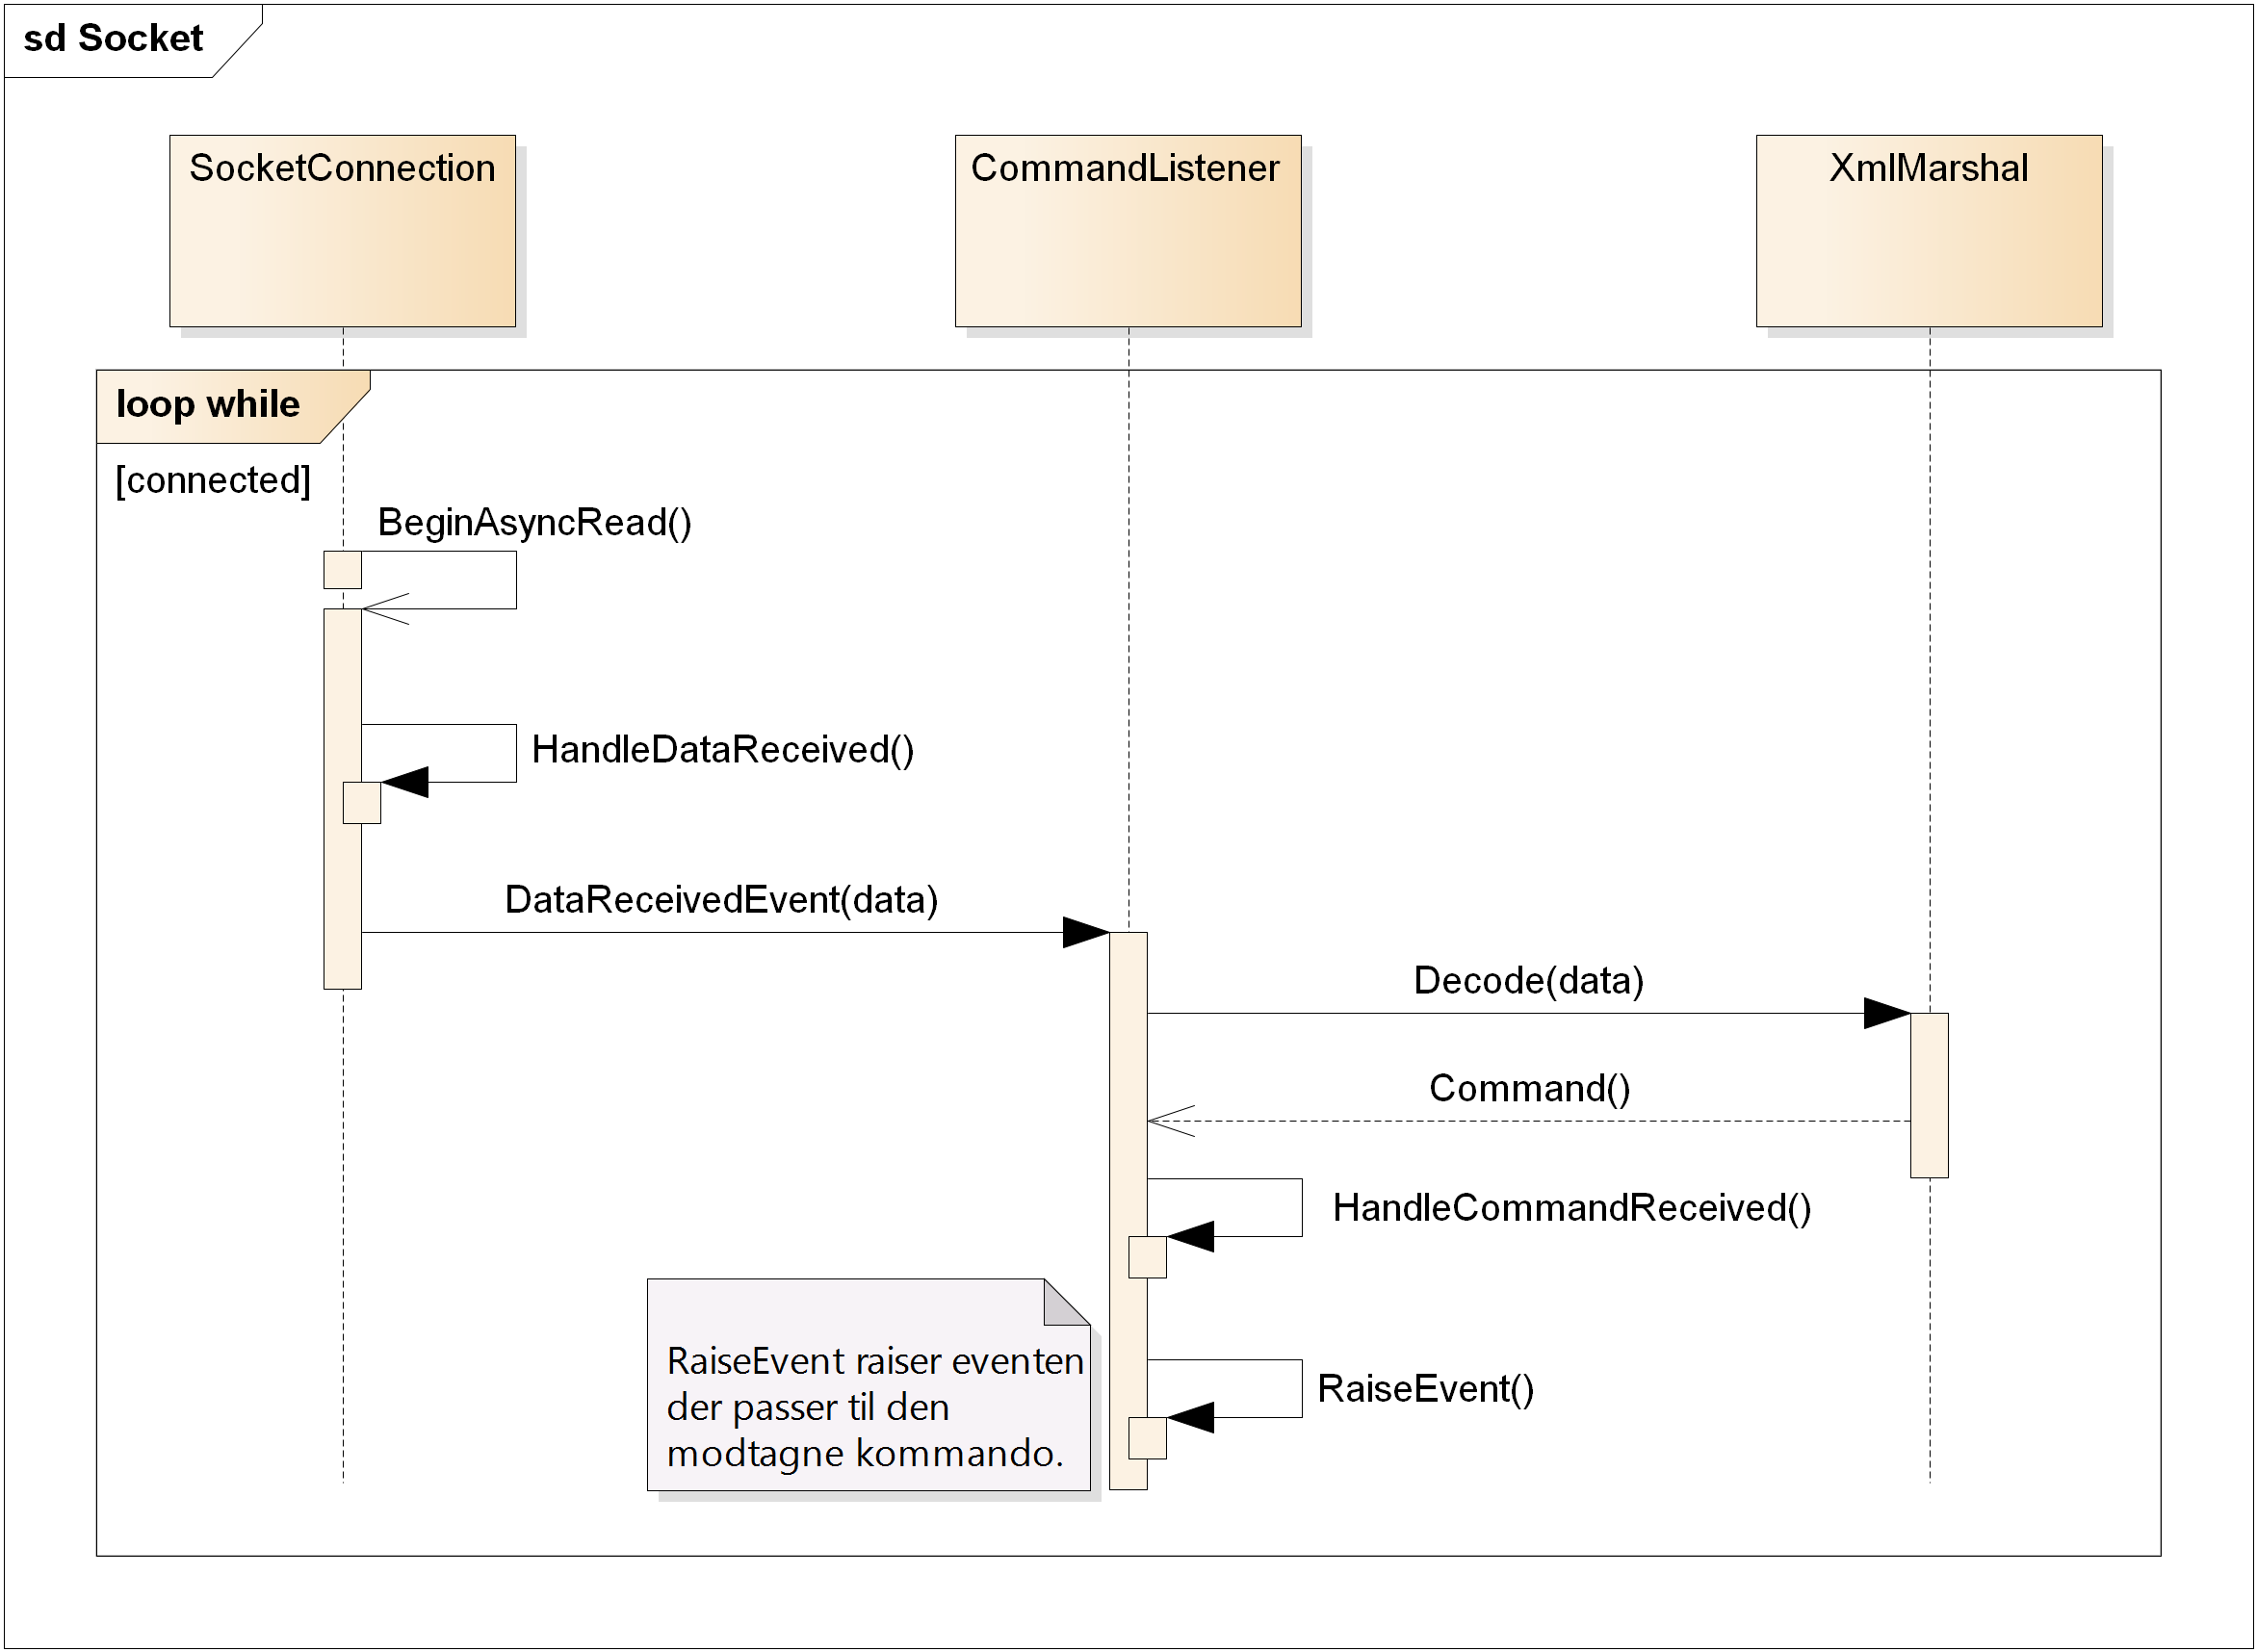
\includegraphics[width=1\textwidth]{Systemdesign/SharedLib/Images/Socket.png}
	\caption{Sekvensdiagram for socketforbindelsen}
	\label{fig:sockit}
\end{figure}

På diagrammet i figur \ref{fig:sockit} ses det hvordan data håndteres. Når den modtages fra serveren. Ved SocketConnection vil read blive ved med at blive kaldt, medmindre der sker en fejl. I dette tilfælde vil et event om fejl blive raised. Se desuden hvordan dataen bearbejdes af modtageren i afsnit \ref{fig:DataReceive} side \pageref{fig:DataReceive}.
 